% Original central-metabolism schematic. Rebuild with: python build.py
\documentclass[10pt,tikz,border=9pt]{standalone}
\usepackage[T1]{fontenc}
\usepackage{helvet}
\renewcommand{\familydefault}{\sfdefault}
\usetikzlibrary{arrows.meta,calc}
\definecolor{ink}{HTML}{1E293B}
\definecolor{muted}{HTML}{536277}
\definecolor{glycolysis}{HTML}{2463A8}
\definecolor{pentose}{HTML}{7952A0}
\definecolor{cycle}{HTML}{A46014}
\definecolor{biosynthesis}{HTML}{137B69}
\definecolor{redox}{HTML}{A53F68}
\definecolor{energy}{HTML}{986300}
\definecolor{quiet}{HTML}{D7DEE7}
\definecolor{surface}{HTML}{FFFFFF}
\ifdefined\darkmode
  \definecolor{ink}{HTML}{E6EDF5}
  \definecolor{muted}{HTML}{B4C1D2}
  \definecolor{glycolysis}{HTML}{7DB9F2}
  \definecolor{pentose}{HTML}{C7A3ED}
  \definecolor{cycle}{HTML}{E9B66D}
  \definecolor{biosynthesis}{HTML}{79CFBA}
  \definecolor{redox}{HTML}{F0A5C2}
  \definecolor{energy}{HTML}{F2CD76}
  \definecolor{quiet}{HTML}{394654}
  \definecolor{surface}{HTML}{121923}
  \pagecolor{surface}
\fi
\begin{document}
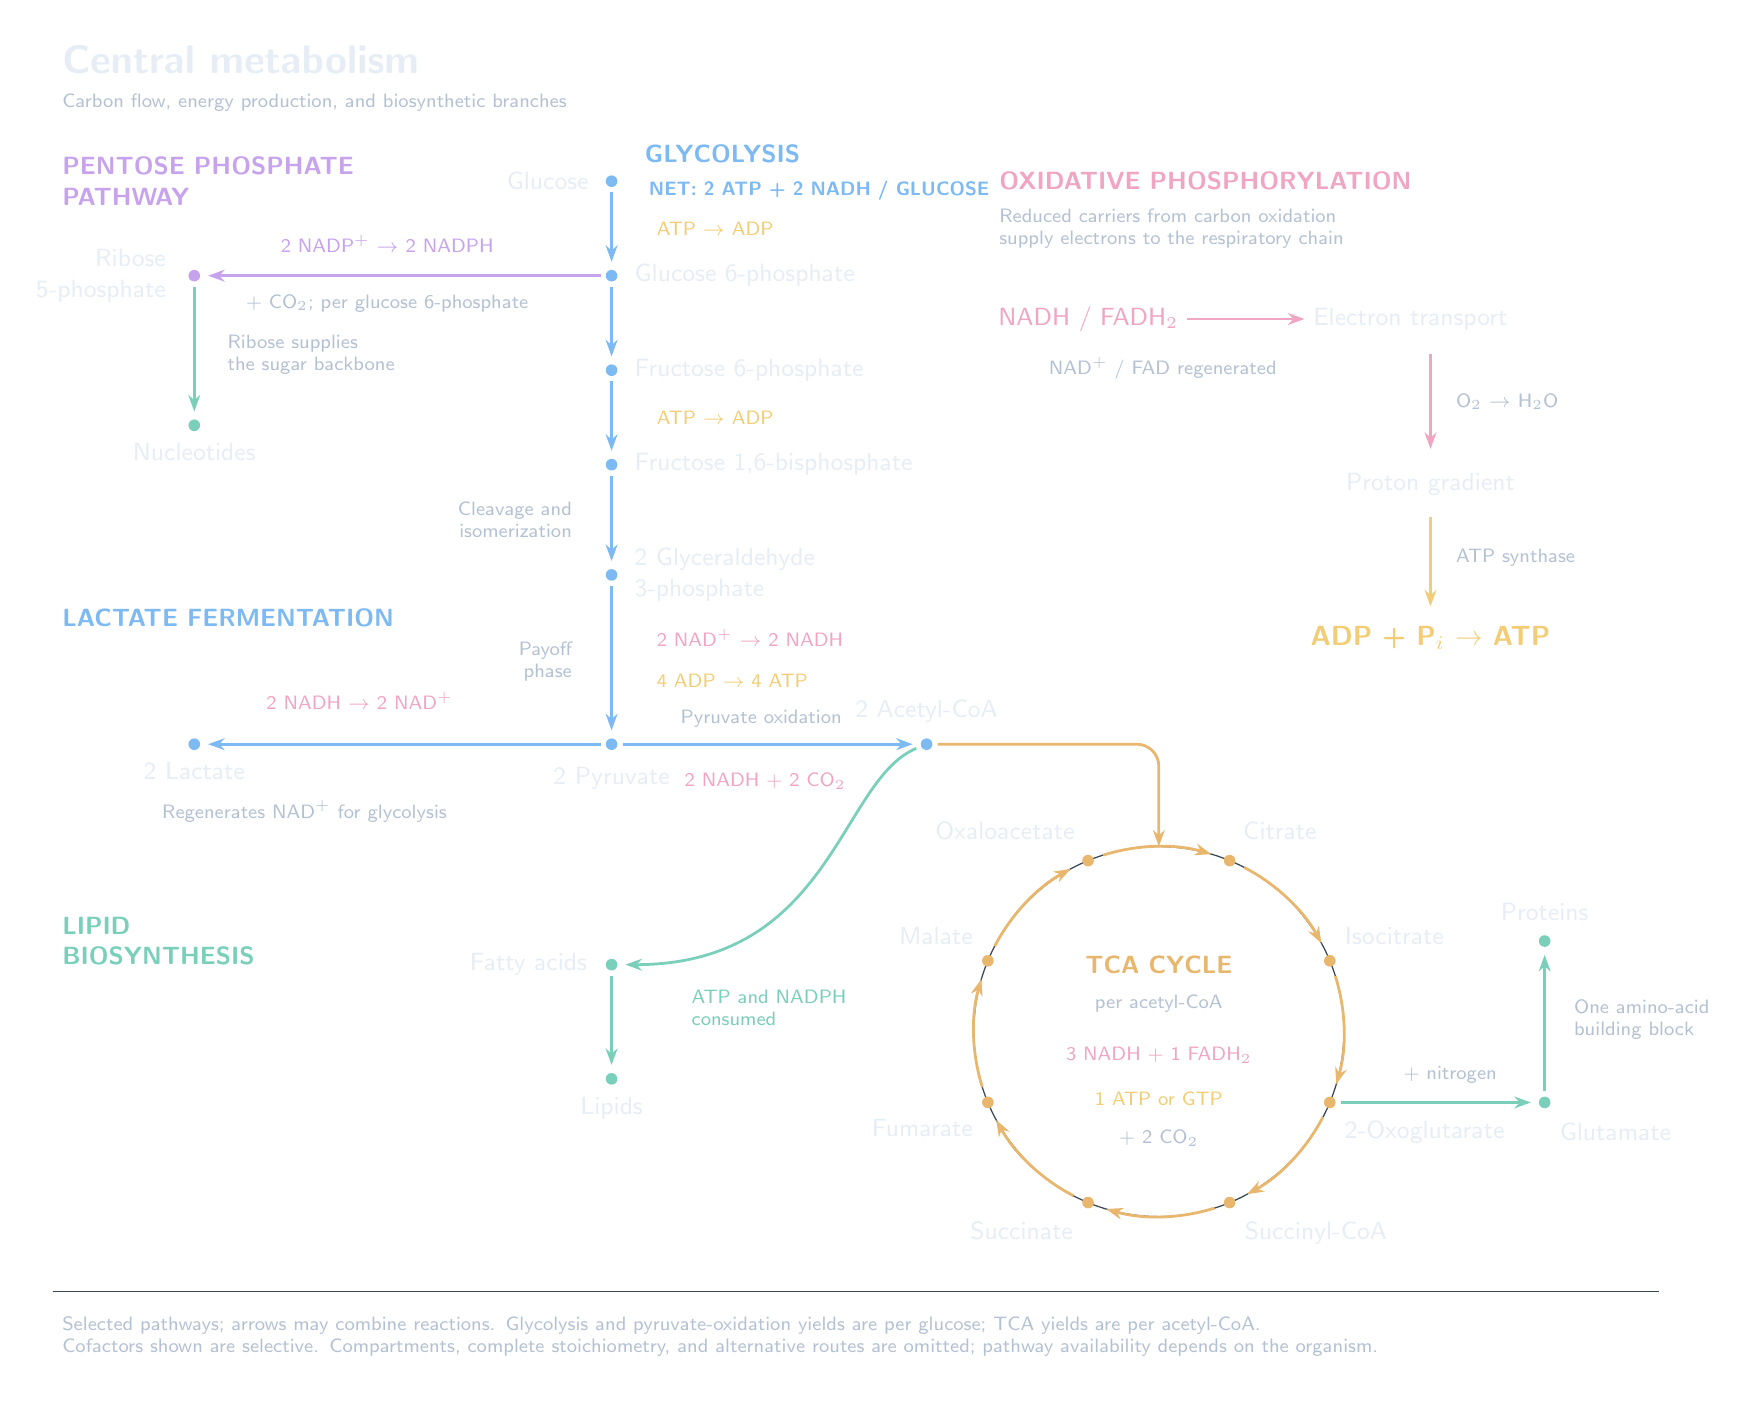
\begin{tikzpicture}[x=1cm,y=1cm,
 every node/.style={font=\sffamily,text=ink},
 label/.style={font=\sffamily\small,inner sep=3pt,align=center},
 heading/.style={font=\sffamily\bfseries\small,align=left},
 smallnote/.style={font=\sffamily\scriptsize,text=muted,align=center},
 cofactor/.style={font=\sffamily\scriptsize,align=center,text=redox},
 route/.style={-{Stealth[length=2.1mm,width=1.5mm]},line width=1.0pt},
 glycolytic/.style={route,draw=glycolysis},
 pentose route/.style={route,draw=pentose},
 tca/.style={route,draw=cycle},
 synthesis/.style={route,draw=biosynthesis}]

% Typography and the margins, rather than enclosing boxes, organize the map.
\node[font=\sffamily\bfseries\Large,anchor=west] at (0.3,14.2) {Central metabolism};
\node[smallnote,anchor=west] at (0.3,13.65) {Carbon flow, energy production, and biosynthetic branches};

% Glycolysis: individual investment steps and the aggregated payoff phase.
\node[heading,text=glycolysis,anchor=west] at (7.7,13.0) {GLYCOLYSIS};
\foreach \name/\yy in {glucose/12.65,g6p/11.45,f6p/10.25,fbp/9.05,gap/7.65,pyruvate/5.50}
  {\coordinate (\name) at (7.4,\yy);}
\foreach \a/\b in {glucose/g6p,g6p/f6p,f6p/fbp,fbp/gap,gap/pyruvate}
  {\draw[glycolytic,shorten <=4pt,shorten >=5pt] (\a)--(\b);}
\foreach \p in {glucose,g6p,f6p,fbp,gap,pyruvate}
  {\fill[glycolysis] (\p) circle[radius=2.1pt];}
\node[label,anchor=east] at ($(glucose)+(-0.18,0)$) {Glucose};
\node[label,anchor=west] at ($(g6p)+(0.18,0)$) {Glucose 6-phosphate};
\node[label,anchor=west] at ($(f6p)+(0.18,0)$) {Fructose 6-phosphate};
\node[label,anchor=west] at ($(fbp)+(0.18,0)$) {Fructose 1,6-bisphosphate};
\node[label,anchor=west,align=left] at ($(gap)+(0.18,0)$) {2 Glyceraldehyde\\3-phosphate};
\node[label,anchor=north] at ($(pyruvate)+(0,-0.18)$) {2 Pyruvate};
\node[cofactor,text=energy,anchor=west] at (7.85,12.05) {ATP $\rightarrow$ ADP};
\node[cofactor,text=energy,anchor=west] at (7.85,9.65) {ATP $\rightarrow$ ADP};
\node[cofactor,anchor=west] at (7.85,6.85) {2 NAD$^+$ $\rightarrow$ 2 NADH};
\node[cofactor,text=energy,anchor=west] at (7.85,6.30) {4 ADP $\rightarrow$ 4 ATP};
\node[smallnote,anchor=east,align=right] at (7.02,8.35) {Cleavage and\\isomerization};
\node[smallnote,anchor=east,align=right] at (7.02,6.55) {Payoff\\phase};
\node[heading,text=glycolysis,anchor=west,font=\sffamily\bfseries\scriptsize] at (7.75,12.53)
  {NET: 2 ATP + 2 NADH / GLUCOSE};

% Pentose branch: yield refers to one G6P routed through the oxidative phase.
\coordinate (r5p) at (2.1,11.45);
\coordinate (nucleotides) at (2.1,9.55);
\draw[pentose route,shorten <=4pt,shorten >=5pt] (g6p)--(r5p);
\fill[pentose] (r5p) circle[radius=2.1pt];
\node[heading,text=pentose,anchor=west] at (0.3,12.65) {PENTOSE PHOSPHATE\\PATHWAY};
\node[cofactor,text=pentose] at (4.55,11.85) {2 NADP$^+$ $\rightarrow$ 2 NADPH};
\node[smallnote] at (4.55,11.10) {+ CO$_2$; per glucose 6-phosphate};
\node[label,anchor=east,align=right] at (1.85,11.45) {Ribose\\5-phosphate};
\draw[synthesis,shorten <=4pt,shorten >=5pt] (r5p)--(nucleotides);
\fill[biosynthesis] (nucleotides) circle[radius=2.1pt];
\node[label,anchor=north] at ($(nucleotides)+(0,-0.12)$) {Nucleotides};
\node[smallnote,anchor=west,align=left] at (2.4,10.45) {Ribose supplies\\the sugar backbone};

% Fermentation returns the reducing equivalents used by glycolysis.
\coordinate (lactate) at (2.1,5.5);
\draw[glycolytic,shorten <=4pt,shorten >=5pt] (pyruvate)--(lactate);
\fill[glycolysis] (lactate) circle[radius=2.1pt];
\node[heading,text=glycolysis,anchor=west] at (0.3,7.10) {LACTATE FERMENTATION};
\node[cofactor] at (4.2,6.05) {2 NADH $\rightarrow$ 2 NAD$^+$};
\node[label,anchor=north] at ($(lactate)+(0,-0.12)$) {2 Lactate};
\node[smallnote] at (3.5,4.65) {Regenerates NAD$^+$ for glycolysis};

% Pyruvate oxidation. Numbers refer to complete oxidation of two pyruvates.
\coordinate (acetyl) at (11.4,5.5);
\draw[glycolytic,shorten <=4pt,shorten >=5pt] (pyruvate)--(acetyl);
\fill[glycolysis] (acetyl) circle[radius=2.1pt];
\node[label,anchor=south] at ($(acetyl)+(0,0.16)$) {2 Acetyl-CoA};
\node[smallnote] at (9.3,5.82) {Pyruvate oxidation};
\node[cofactor] at (9.35,5.03) {2 NADH + 2 CO$_2$};

% Fatty-acid synthesis branches from the acetyl-CoA pool.
\coordinate (fatty) at (7.4,2.70);
\coordinate (lipids) at (7.4,1.25);
\draw[synthesis,shorten <=4pt,shorten >=5pt] (acetyl)
  .. controls (10.3,5.05) and (10.2,2.7) .. (fatty);
\fill[biosynthesis] (fatty) circle[radius=2.1pt];
\node[label,anchor=east] at ($(fatty)+(-0.2,0)$) {Fatty acids};
\node[cofactor,text=biosynthesis,align=left] at (9.4,2.15) {ATP and NADPH\\consumed};
\draw[synthesis,shorten <=4pt,shorten >=5pt] (fatty)--(lipids);
\fill[biosynthesis] (lipids) circle[radius=2.1pt];
\node[label,anchor=north] at ($(lipids)+(0,-0.12)$) {Lipids};
\node[heading,text=biosynthesis,anchor=west] at (0.3,3.0) {LIPID\\BIOSYNTHESIS};

% TCA cycle: all coordinates use one radius. The arrows are genuine circular arcs.
\coordinate (center) at (14.35,1.85);
\def\radius{2.35}
\draw[draw=quiet,line width=0.45pt] (center) circle[radius=\radius];
\foreach \name/\angle in {oaa/112.5,citrate/67.5,isocitrate/22.5,akg/-22.5,succoa/-67.5,succinate/-112.5,fumarate/-157.5,malate/-202.5}{
  \coordinate (\name) at ($(center)+(\angle:\radius)$);
  \fill[cycle] (\name) circle[radius=2.1pt];
  \pgfmathsetmacro{\start}{\angle-5}
  \pgfmathsetmacro{\finish}{\angle-39}
  \draw[tca] ($(center)+(\start:\radius)$) arc[start angle=\start,end angle=\finish,radius=\radius];
}
\node[label,anchor=south east] at ($(oaa)+(-0.06,0.15)$) {Oxaloacetate};
\node[label,anchor=south west] at ($(citrate)+(0.06,0.15)$) {Citrate};
\node[label,anchor=south west] at ($(isocitrate)+(0.08,0.10)$) {Isocitrate};
\node[label,anchor=north west] at ($(akg)+(0.08,-0.12)$) {2-Oxoglutarate};
\node[label,anchor=north west] at ($(succoa)+(0.08,-0.14)$) {Succinyl-CoA};
\node[label,anchor=north east] at ($(succinate)+(-0.08,-0.14)$) {Succinate};
\node[label,anchor=north east] at ($(fumarate)+(-0.08,-0.1)$) {Fumarate};
\node[label,anchor=south east] at ($(malate)+(-0.08,0.1)$) {Malate};
\draw[tca,rounded corners=8pt,shorten <=4pt] (acetyl)--(14.35,5.5)--($(center)+(90:\radius)$);
\node[heading,text=cycle,align=center] at (14.35,2.70) {TCA CYCLE};
\node[smallnote] at (14.35,2.20) {per acetyl-CoA};
\node[cofactor] at (14.35,1.55) {3 NADH + 1 FADH$_2$};
\node[cofactor,text=energy] at (14.35,1.0) {1 ATP or GTP};
\node[smallnote] at (14.35,0.50) {+ 2 CO$_2$};

% A direct biosynthetic exit from the TCA carbon skeletons.
\coordinate (glutamate) at (19.25,0.95);
\coordinate (protein) at (19.25,3.0);
\draw[synthesis,shorten <=4pt,shorten >=5pt] (akg)--(glutamate);
\fill[biosynthesis] (glutamate) circle[radius=2.1pt];
\node[label,anchor=north west] at ($(glutamate)+(0.08,-0.15)$) {Glutamate};
\draw[synthesis,shorten <=4pt,shorten >=5pt] (glutamate)--(protein);
\fill[biosynthesis] (protein) circle[radius=2.1pt];
\node[label,anchor=south] at ($(protein)+(0,0.15)$) {Proteins};
\node[smallnote,anchor=west,align=left] at (19.5,2.0) {One amino-acid\\building block};
\node[smallnote] at (18.05,1.30) {+ nitrogen};

% Respiration has its own compact, aligned explanation of the energy connection.
\node[heading,text=redox,anchor=west] at (12.2,12.65) {OXIDATIVE PHOSPHORYLATION};
\node[smallnote,anchor=west,align=left] at (12.2,12.05) {Reduced carriers from carbon oxidation\\supply electrons to the respiratory chain};
\node[label,text=redox,anchor=west] (donors) at (12.2,10.90) {NADH / FADH$_2$};
\node[label,anchor=west] (etc) at (16.2,10.90) {Electron transport};
\draw[route,draw=redox] (donors.east)--(etc.west);
\node[smallnote] at (14.4,10.27) {NAD$^+$ / FAD regenerated};
\draw[route,draw=redox] (17.8,10.45)--(17.8,9.25);
\node[smallnote,anchor=west] at (18.0,9.85) {O$_2$ $\rightarrow$ H$_2$O};
\node[label] (gradient) at (17.8,8.8) {Proton gradient};
\draw[route,draw=energy] (17.8,8.38)--(17.8,7.25);
\node[smallnote,anchor=west] at (18.0,7.87) {ATP synthase};
\node[label,text=energy,font=\sffamily\bfseries] at (17.8,6.85) {ADP + P$_i$ $\rightarrow$ ATP};

% Reuse-safe scope and counting convention.
\draw[draw=quiet,line width=0.5pt] (0.3,-1.45)--(20.7,-1.45);
\node[smallnote,anchor=north west,align=left,text width=20cm] at (0.3,-1.65)
 {Selected pathways; arrows may combine reactions. Glycolysis and pyruvate-oxidation yields are per glucose; TCA yields are per acetyl-CoA.\\
 Cofactors shown are selective. Compartments, complete stoichiometry, and alternative routes are omitted; pathway availability depends on the organism.};
\path[use as bounding box] (0,-2.6) rectangle (21,14.6);
\end{tikzpicture}
\end{document}
